Having laid the theoretical framework, we come to the practical part of this thesis --- a proof-of-concept implementation of multiple affective agents interacting with each other. This section contains the following parts: (1) the world in which act, (2) the architecture of these agents, and (3) the evolutionary changes in the agent pool from generation to generation.

\subsection{World}

The choice of world profoundly affects the implementation of the agent: its knowledge base, mechanism of perception and interaction, the required complexity of the implementation, etc. On one hand, the world should be simple enough to permit a reasonably small and effective agent which does not have to solve hard AI problems (like human-level sight) to deal with what we, in this context, might call details --- but on the other, the world should be sufficiently complex to allow the agent to shine. This is especially true in the case of an affective agent whose actions should be visibly influenced in rich and subtle ways by its emotional state. I shall first lay out the design goals and then evaluate three possible worlds for agents.

\paragraph{Design goals} The two most important criteria for prospective worlds are richness of interaction and world complexity, in that order. As said, an evaluation of affective agents is only possible if they can interact with their environment and other entities in a sufficiently complex way to allow agents with different emotional profiles to be distinguished from each other. Mechanisms of problem-solving like STRIPS \cite{fikesNilsson}, A* \cite{nilssonAStar}, ASP \cite{lifschitz}, forward-/backward-planning, etc. have been explored in the context of structurally simple worlds, generally those representable through propositional logic, cost-functions, decision tress, and the like. While these are useful, they are less appropriate in an affective scenario for the following two reasons:

\begin{enumerate}
	\item they are geared towards finding provably optimal solutions to computationally expensive but conceptually simple problems like planning or game-playing and
	\item they rely heavily on hand-crafted ontologies and domain knowledge on the part of the human programmer.
\end{enumerate}

For a world to be useful to us and to avoid these pitfalls, it should be in some sense realistic: it should permit a large number of different kinds of interactions, and it should not provide agents in it with perfect knowledge about its rules. 

I admit that I here stand in opposition with Marvin Minsky, who famously recommended the use of idealized micro-worlds to study artificial intelligence, in that same vein in which physics makes use of ideal, frictionless planes and perfect spheres. His argument certainly has merit, but I believe that emotion is too complex a phenomenon for such abstract scenarios. In too simple a setting, pure reasoning not only easily outperforms emotional behaviour, but avenues for exhibiting emotional behaviour are scarce to begin with. For this reason, I propose that, in this context, rich interactions should take precedence over idealization and simplicity.

It is of course still desirable to minimize complexity as far as possible. An overwhelmingly complex world has two obvious drawbacks: first, the required complexity of an agent scales with the complexity of the world; second, the more complex the world, the harder it is to reason about it. If there are a hundred ways to succeed, for instance, agent performance becomes quite difficult to measure.

\subsubsection{Blocks world}

Blocks worlds are the simplest type of abstract world, and many variations exist. They all have in common a number of shapes placed on top of each other in a 2-dimensional world. An agent can pick up and move a shape if and only if there are no other shapes on top of it (and if it is not already holding one). The goal generally consists of achieving some desired configuration of shapes, such as building or piecewise transporting a tower, or collecting all red triangles. 

Micro-worlds like blocks worlds have extensively studied. In this, their simplicity has been their great advantage --- That very simplicity is serious problem for us, however. Affect is inherently a subtle and social phenomenon; it is not clear how it could be believably exhibited in such an abstract and simple world. The very same properties which expedite their theoretical study make them useless for our evaluation.

%\subsubsection{Real world}

\subsubsection{Wumpus world}

The traditional Wumpus world, as described in Russell and Norvig's {\em Artificial Intelligence: A Modern Approach} \cite[p. 236]{norvig}, is a grid-based, 4x4 cave world with one agent, one monster --- the Wumpus --- and gold placed in random rooms. The agent starts at position $\langle 1,1\rangle$ and can move forward or turn 90$^\circ$ to the left or right. If it enters a room with a pit or a live Wumpus, it dies; its goal is to find and collect the gold and then move back to position $\langle 1,1\rangle$ to climb out of the cave. In addition, it has one arrow which he can fire straight ahead to defend against the Wumpus. The agent has only the following local information \cite[p. 237]{norvig}:
\begin{itemize}
	\item In the square containing the Wumpus and in the directly (not diagonally) adjacent squares, the agent will perceive a {\em Stench}.
	\item In the squares directly adjacent to a pit, the agent will perceive a {\em Breeze}.
	\item In the square where the gold is, the agent will perceive a {\em Glitter}.
	\item When an agent walks into a wall, it will perceive a {\em Bump}.
	\item When the Wumpus is killed, it emits a woeful {\em Scream} that can be perceived anywhere in the cave.
\end{itemize}

This type of world is simple enough to be amenable to rule-based reasoning, although it can contain ambiguous situations where the agent does not have enough information to make the best choice. For example, if an agent moves to position $\langle p_x,p_y \rangle$ and experiences a breeze, 1, 2, or 3 adjacent rooms may contain pits, but it cannot be safely determined which ones these are. Thus,  occasionally, the agent must choose between climbing out without the gold and risking death by pit or Wumpus.

For our purposes, this is a bit too simple, however. Caution/bravery is the only axis along which agents can be differentiated and although various complex behaviours --- such as trying one dangerous cell, then going back and trying another one to explore the world --- are possible, these do not have a clear relation to emotional states.

Let us, while staying true to the spirit of the original, now define a type of extended Wumpus world \wext\ that allows more varied interaction between agent an environment.

\begin{definition}[\wext-type world]\label{def:wext}
	Let $\type{T_v}$, $\type{T_e}$, $\type{T_g}$ be arbitrary types. Further, let $G$ be a directed graph with vertex labels of type $\type{T_v}$ and edge labels of type $\type{T_e}$, and let $\mathrm{gl}$ be an object of type $\type{T_g}$. Then the tuple \tuple{G, \mathrm{gl}} is a \wext-type world \paren{with type parameters $\type{T_v}$, $\type{T_e}$, $\type{T_g}$}. We call $G$ the {\em world frame} and $\mathrm{gl}$ the {\em world data}.
\end{definition}

We can interpret each vertex $v$ in the graph as a room with attached data $l(v)$ of type $\type{T_v}$, and each edge $e$ as an unidirectional connection between rooms with attached data (such as path costs) $l(e)$ of type $\type{T_e}$. $\mathrm{gl}$ is the global world data. Next, we specify some properties of the world frame:

\begin{definition}[World properties]
	Let $W = \tuple{G,\mathrm{gl}}$ be a \wext-world. We say that $W$ has property $X$ iff it fulfils the first-order sentence corresponding to $X$. The following properties are of importance:
	
	

	\begin{center}
		\begin{tabular}[b]{l l}
		\toprule
		\textbf{Property name} & \textbf{FO sentence}\\
		\midrule\addlinespace[0.7em]
		Reflexive & $\allQ{v \in V(G)} (v,v) \in E(G)$\\ \addlinespace[0.7em]
		Non-Euclidean &
		\begin{minipage}[t]{0.65\textwidth}
			$\allQ{\textit{ pairwise distinct } v_1,v_2,v_3 \in V(G)}$\\$\{(v_1,v_2),(v_1,v_3)\} \subseteq E(G) \Rightarrow (v_2,v_3) \notin E(G)$
		\end{minipage}\\ \addlinespace[0.7em]
		Symmetrical & $\allQ{v_1,v_2 \in V(G)} (v_1,v_2) \in E(G) \Rightarrow (v_2,v_1) \in E(G)$\\ \addlinespace[0.7em]
		Connected & $\allQ{v_1,v_2 \in V(G)}$ there exists a path from $v_1$ to $v_2$ in $G$\\ \addlinespace[0.7em]
		
		$n$-dimensionally embeddable
		 &
		\begin{minipage}[t]{0.65\textwidth}
		there exists an infinite graph $S$ such that
		\begin{enumerate}
			\item $V(G) \subseteq V(S)$,
			\item $E(G) \subseteq E(S) \cup \{ (v,v)\ |\ (v,v) \in E(G) \}$,
			\item $S$'s drawing, embedded into $\R^n$, forms a regular tiling, and
			\item $(v_1,v_2) \in E(S)$ iff the distance between $v_1$ and $v_2$ in $\R^n$ is 1.
		\end{enumerate}
		\end{minipage}
		
		\\ \addlinespace[0.5em]
		\bottomrule
		
		\end{tabular}
	\end{center}
\end{definition}

The first four properties speak for themselves. As for the fifth --- Figure~\ref{fig:2dgrid} shows an example of a 2-dimensionally embeddable frame. A frame $G$ is $n$-dimensionally embeddable if it is a fragment of an infinite, $n$-dimensional, square grid of nodes $S$, plus any loops $G$ might have. When we embed this infinite grid $S$ into $\R^n$ through an embedding, every edge corresponds to a vector of length 1 along exactly one dimension. If we additionally take $G$'s loops to correspond to null-vectors, this induces an {\em edge direction function} and a {\em position function}:

\begin{definition}[Edge direction and position]
Let $W = \tuple{G, \mathrm{gl}}$ be an $n$-dimensionally embeddable world (for some $n$) and $\epsilon$ an embedding of $W$ into $\R^n$. Then we have an {\em edge direction function} 

$$\Delta_n^\epsilon : E(G) \rightarrow \{0,x_1^+,x_1^-,x_2^+,x_2^-,\dots,x_n^+,x_n^-\}$$

with $0$ corresponding to a loop and $x_i^+$/$x_i^-$ corresponding to forward/backward movement in the $i$th dimension. We also have a {\em position function}

$$\pi^\epsilon : V(G) \rightarrow \R^n.$$

When the number of dimensions and the embedding are obvious, we omit $n$ and $\epsilon$.
Since $\pi^\epsilon$ is injective, an inverse $(\pi^\epsilon)^{-1}$ also exists. Through it, we define the {\em indexing function} of $W$:

$$
	\begin{array}{l}
		[] : n\textit{-dimensionally embeddable world} \rightarrow \R^n \rightarrow \type{Maybe}\ V(G)\\
		W[p] \equiv \left\{
			\begin{array}{l l}
				\type{Just } (\pi^\epsilon)^{-1}(p) & \textit{if } (\pi^\epsilon)^{-1}(p) \textit{ is defined}\\
				\type{Nothing} & \textit{otherwise}
			\end{array}
			\right.
	\end{array}
$$
\end{definition}

We will give agents access to $\Delta_n^\epsilon$ and $\pi^\epsilon$ (or simply $\Delta$ and $\pi$) to allow them to determine their position and direction in the world. Providing such information might seem problematic, but we thereby free ourselves from having to insert things like landmarks, wind currents, stars, and other navigational aids into the world. Given that navigation is not the focus of this thesis, this seems an appropriate simplification. Using the above properties, we can specify a subtype of \wext-type worlds:

\begin{figure}
	\centering
		\begin{tikzpicture}[scale=0.8]
		\draw (1,1) -- (5,1); \draw (7,1) -- (10,1);
		\draw (0,2) -- (10,2);
		\draw (0,3) -- (1,3); \draw (2,3) -- (4,3); \draw (6,3) -- (10,3);
		\draw (0,4) -- (1,4); \draw (2,4) -- (4,4); \draw (6,4) -- (7,4); \draw (8,4) -- (9,4);
		\draw (0,5) -- (1,5); \draw (2,5) -- (5,5);
		\draw (0,6) -- (5,6); \draw (8,6) -- (9,6);
		\draw (0,7) -- (2,7); \draw (4,7) -- (6,7); \draw (7,7) -- (10,7);
		\draw (0,8) -- (2,8); \draw (3,8) -- (10,8);
		\draw (3,9) -- (10,9);
		
		\draw (1,1) -- (1,2); \draw (1,3) -- (1,5); \draw (1,6) -- (1,8);
		\draw (2,0) -- (2,5); \draw (2,6) -- (2,8);
		\draw (3,0) -- (3,10);
		\draw (4,1) -- (4,10);
		\draw (5,0) -- (5,2);
		\draw (5,5) -- (5,10);
		\draw (6,2) -- (6,4); \draw (6,7) -- (6,10);
		\draw (7,1) -- (7,4); \draw (7,7) -- (7,10);
		\draw (8,0) -- (8,10);
		\draw (9,0) -- (9,6); \draw (9,7) -- (9,10);
	\end{tikzpicture}
	\caption{A segment of 2-dimensionally embeddable world. The vertices are its rooms, the edges are the connections between the rooms.}
	\label{fig:2dgrid}
\end{figure}

\begin{definition}[2D grid world]
	Let $W = \tuple{G,\mathrm{gl}}$ be a \wext-type world \paren{with type variables $\type{T_v}, \type{T_e}, \type{T_g}$}. If $W$ is reflexive, connected, and 2-dimensionally embeddable $W$ is a {\em 2D grid world}.
	Every 2D grid world has an associated function $\Delta_2 : E(G) \rightarrow \{0,x_1^+,x_1^-,x_2^+,x_2^- \}$.\\
	Note: every $n$-dimensionally embeddable world is also symmetrical and non-Euclidean.
\end{definition}

Grid worlds, as we have seen, are potentially infinite, n-dimensional grids, although their cells need not form a square or cube. Their shape can be irregular in that some rooms and connections may be missing, as long as the shape as a whole stays connected.

2D grid worlds are representationally the same as \wext-type worlds; they just have some structural invariants on their frames. If we additionally specialize the representation through the type parameters $\type{T_v}$, $\type{T_e}$, and $\type{T_g}$, we arrive at the type of world which will serve as the environment for our agents: the ``jungle world'' \wjun.

\begin{definition}[\wjun]
\label{def:wjun}
Let $\type{T_v}$, $\type{T_e}$, $\type{T_g}$ be the following tuples:

$$
	\begin{array}{r c l}
		\type{TV_{\mathrm{jun}}} & = & \langle \field{agents} :: [\type{Agent}],\\
		           &   &       \ \field{wumpus} :: [\type{Wumpus}],\\
		           &   & 	   \ \field{plants} :: \type{Maybe\ Plant},\\
		           &   &       \ \field{stench} :: \R,\\
		           &   &       \ \field{breeze} :: \R,\\
		           &   &	   \ \field{pit}    :: \B,\\
		           &   &	   \ \field{gold}   :: \N \rangle 
		\\
		\\
		\type{TE_{\mathrm{jun}}} & = & \langle \field{danger} :: \R,\\
				   &   &       \ \field{fatigue} :: \R \rangle
		\\
		\\
		\type{Temp} & = & \type{Freezing} + \type{Cold} + \type{Temperate} + \type{Warm} + \type{Hot}\\
		\\
		\type{TG_{\mathrm{jun}}} & = & \langle \field{time} :: \N,\\
				   &   &       \ \field{temperature} :: \type{Temp} \rangle
	\end{array}
$$

$\type{Agent}$ and $\type{Wumpus}$ are the following records:

$$
	\begin{array}{r c l}
		\type{Item} & = & \type{Gold + Fruit + Meat}\\
		\\
		\type{Agent} & = & \langle \field{name} :: \type{String},\\ 
					 & = & \ \field{direction} :: \type{X_1^+ + X_1^- + X_2^+ + X_2^-},\\
					 &   & \ \field{health} :: \R,\\
					 &   & \ \field{fatigue} :: \R,\\
					 &   & \ \field{inventory} :: [\type{\langle Item, \N \rangle}] \rangle
		\\
		\\
		\type{Wumpus} & = & \langle \field{health} :: \R,\\
					  &   & \ \field{fatigue} :: \R\rangle
	\end{array}
$$

Further, let $\mathrm{gl}$ be a value of type $\type{TG}_{\mathrm{jun}}$ and let $G$ be any 2D grid world with node labels of type $\type{TV}_{\mathrm{jun}}$ and edge labels of type $\type{TE}_{\mathrm{jun}}$. Then, $\tuple{G, \mathrm{gl}}$ is a \wjun-type jungle world.
\end{definition}

Although the field names are suggestive of the way in which a \wjun-type world works, the type, strictly speaking, only specifies the data and frame properties. We can employ such worlds in any sort of scenario, with whatever semantics we wish. Notwithstanding, our implementation will use a straightforward {\em standard semantics}, defined below.

\begin{definition}[Semantics and runs of \wjun-type worlds]
Let $\varphi$ be a function of type $\wjun \rightarrow \wjun$. $\varphi$ is called {\em semantics of \wjun-type worlds}.
Let $W$ be a \wjun-type world. The iterated application of $\varphi$ to $W$, given by the list ${[W, \varphi(W), \varphi^2(W), \varphi^3(W), \dots]}$, is called a {\em run of $W$ \paren{with semantics $\varphi$}}. $\varphi^n(W)$ is referred to as the {\em state of $W$'s simulation at time $n$ \paren{with semantics $\varphi$}}.
\end{definition}

\begin{definition}[Standards semantics of \wjun-type worlds]
\label{def:ssem}
The standard semantics for \wjun-type worlds are given by the function $\ssem :: \type{\wjun \rightarrow \wjun}$. $\ssem$ is defined as 
$$\ssem(W = \tuple{G, \mathrm{gl}}) = \tuple{G', \mathrm{gl}'}, $$
where $W'$ is identical to $W$, except for the following changes.\\

\begin{description}
	\item[Environment] For all $v \in V(G)$, perform the following:
	
	\begin{description}
		\item[Wumpus.] If there is a Wumpus in a cell $w$ at $\leq 3$ distance from $v$, increase $v$'s stench by
		$$
			\frac{
				\log_{3}(3 - \dist{v}{w}) - \field{stench}(l(v))
			}{2}
		$$
		If there is no Wumpus within distance $\leq 3$, decrease $v$'s stench by $\frac{1}{3}$, to a minimum of 0.
		
		\item[Plant.] If there is a plant on $v$ and it has no fruit, increase its growth by $\frac{1}{10}$. If its growth thereby reaches $1$, add a fruit to the plant and reset the growth to 0.
		
		\item[Pit] If there is a pit in a cell $w$ at a distance $\leq 3$ from $v$, set the breeze to
 		$$
			\log_{3}(3 - \dist{v}{w})
		$$
	\end{description}
	
	\item[Global data] The {\em daylight function} is defined as
	
	$$
			\field{cycle}(t) = 
			\left\{
				\begin{array}{l l l l}
					0 & \mt{if } & 20 & \leq |n - 25|\\
					1 & \mt{if } & 15 & \leq |n - 25| < 20\\
					2 & \mt{if } & 10 & \leq |n - 25| < 15\\
					3 & \mt{if } & 5 & \leq |n - 25| < 10\\
					4 & \mt{if } & & \ \ \ |n - 25| < 5
				\end{array}
			\right.
	$$
	
	The new global data $\mathrm{gl}'$ are given by
	
	$$
		\begin{array}{r c l}
			\mathrm{gl}' & = & \langle \field{time}(\mathrm{gl}) + 1\ \mathrm{mod}\ 50,\\
					   &   &       \ \field{cycle} \circ \field{temperature}(\mathrm{gl}') \rangle\\
			\\
			\field{cycle}(t) & = &
			\left\{
				\begin{array}{l l}
					\type{Freezing} & \mt{if }\ \field{light}(t) = 0\\
					\type{Cold} & \mt{if }\ \field{light}(t) = 1\\
					\type{Temperate} & \mt{if }\ \field{light}(t) = 2\\
					\type{Warm} & \mt{if }\ \field{light}(t) = 3\\
					\type{Hot} & \mt{if }\ \field{light}(t) = 4
				\end{array}
			\right.\\
		\end{array}
	$$
	
	\item[Wumpus behavior] Every Wumpus has three behaviors:
	
	\begin{enumerate}
		\item If the Wumpus is adjacent to a player, it performs the \action{attack} action on that player.
		
		\item If there is a player reachable with at most $\field{light} \circ \field{time} (\mathrm{gl})$ edges, move along the edge that minimizes the distance to that player (in $\R^2$). If there are multiple players, choose one at random as target. This target choice remains until the player is no longer within range.
		
		\item If there is no player within range, move in a random direction with probability
		
		$$
			0.2 \times (1 + \field{light} \circ \field{temperature} (\mathrm{gl})).
		$$
	\end{enumerate}
	
	Whenever a Wumpus travels along an edge $e$ with $\Delta(e) \neq 0$, apply $0.1$ damage with probability $\field{danger}(e)$.
	
	\item[Agent behavior] Agents always move after Wumpuses and, depending on their implementation, may choose one of the following actions:
	
	\begin{enumerate}
		\item[\action{move}] --- move along an edge $e$. If $\Delta(e) = 0$, restore $0.1$ of the agent's fatigue, otherwise reduce it by $0.05 \times \field{fatigue}(e)$. Additionally (if $\Delta(e) \neq 0$), apply $0.1$ damage with probability $\field{danger}(e)$.
		
		If an agent's fatigue is below $0.2$, it cannot choose this action.
		
		\item[\action{rotate}] --- the agent changes the direction into which it is facing to a value in ${x_1^+,x_1^-,x_2^+,x_2^-}$.
		
		\item[\action{attack}] --- move along an edge $e$ to attack an agent or wumpus.
		
		\item[\action{give}] --- give an item $i$ from the agent's inventory to another agent $a$.
		
		\item[\action{gather}] --- if there is a plant with a fruit on the agent's cell, take the fruit and put it in the agent's inventory.
		
		\item[\action{butcher}] --- if there is a dead Wumpus on the agent's cell, remove it and add an item of meat to the agent's inventory.
		
		\item[\action{collect}] --- if there is $n$ gold on the player's cell, take an amount $m$ ($1 \leq m \leq n$) of it an put it into the agent's inventory.
		
		\item[\action{eat}] --- eat a meat- or fruit-item $i$ from the agent's inventory. Restore $0.5$ health.
		
		\item[\action{gesture}] --- expresses a gesture in the form of a string $s$. All other agents on the same cell receive $s$.
	\end{enumerate}
	
\end{description}
\end{definition}

It should now be clear why \wjun\ is called a jungle world: it is a social hunter-gatherer scenario in which uncoordinated agents act and interact without any explicit performance measure. They can gather food or gold, rest, hunt wumpuses, communicate via gestures, and even develop friendships, but fundamentally, everyone is out for himself. The goal of simulating affective agents in such a world is to see which behavioural profiles are successful, how they develop over multiple generations, and how they engage each other.

\subsection{Agents}

The agents of our simulation are composed of two parts: their minds and their bodies. Their minds constitute their sensors and agents functions; their bodies, make up their actuators, although they are more than that. An agent's body can be damaged and healed, perceived by others, and it can hold items. As such, the bodies are actually part of the world. From the point of view of the agent's mind, they are external objects they happen to control.

\subsubsection{Body and percepts}

As we saw in Definitions~\ref{def:wjun} and \ref{def:ssem}, agents (1) have a body composed of a name, health, fatigue, and an inventory of items they carry, and (2) can execute one of a fixed set of actions at each step. These data function in the obvious way: the name is publicly available information other agents can use for identification, the agent is killed when its health drops to zero, fatigue determines the effectiveness when attacking and prevents movement when low, and the inventory is used to store items which the agent can use for itself or give away to others.

What we are missing is the description of the agent's percepts in the world. As in the original Wumpus world, an agent can perceive everything on its cell:
	\begin{enumerate}
		\item the list other agents,
		\item the list of (dead) Wumpuses,
		\item the plant, if present,
		\item the breeze,
		\item the stench, and
		\item the amount of gold.
	\end{enumerate}
	
In addition to this local information, the agent also has a sense of sight, modelled via an approximately $\frac{\pi}{2}$ radians cone, the length of which depends on daylight. Formally:

\begin{definition}[Sight cone]
	\label{def:los}
	Let $W = \tuple{G, \mathrm{gl}}$ be a 2D grid world. Let an agent be on vertex $v \in V(G)$, facing into direction $d$. Let further $l_d$ be the line starting at $v$ and extending infinitely into direction $d$, and $l_{v,w}$ be the line from $v$ to $w$. Then, any other vertex $w \in V(G)$ falls into the agent's sight cone exactly if:
	
	\begin{enumerate}
		\item the angle between $l_{v,w}$ and $l_d$ is $\leq \frac{\pi}{4}$,
		\item $\dist{v}{w} \leq 1.5 \times (\field{light} \circ \field{time} (\mathrm{gl}) + 1)$, and
		\item there is a path $v_1, v_2, \dots, v_n$ from $v$ to $w$ in $G$ such that
		the distance between $v_i$ and the closest point along $l_{v,w}$ is $\leq \frac{\sqrt{2}}{2}$ ($1 \leq i \leq n$).
	\end{enumerate}
\end{definition}

Criterion one restricts the sight cone to $\frac{\pi}{4}$ radians; criterion two limits its length based on light conditions; criterion three demands rough line-of-sight, saying that the path in $G$ may never deviate more than one cell from the line in $\R^2$. Figure~\ref{fig:los} illustrates the working of this mechanism.
%
\begin{figure}
	\centering
		\begin{tikzpicture}[scale=0.80]
		\draw (1,-1) -- (5,-1); \draw (7,-1) -- (10,-1);
		\draw (0,-2) -- (10,-2);
		\draw (0,-3) -- (1,-3); \draw (2,-3) -- (4,-3); \draw (6,-3) -- (10,-3);
		\draw (0,-4) -- (1,-4); \draw (2,-4) -- (4,-4); \draw (6,-4) -- (7,-4); \draw (8,-4) -- (9,-4);
		\draw (0,-5) -- (1,-5); \draw (2,-5) -- (5,-5);
		\draw (0,-6) -- (5,-6); \draw (8,-6) -- (9,-6);
		\draw (0,-7) -- (2,-7); \draw (4,-7) -- (6,-7); \draw (7,-7) -- (10,-7);
		\draw (0,-8) -- (2,-8); \draw (3,-8) -- (10,-8);
		\draw (3,-9) -- (10,-9);
		
		\draw (1,-1) -- (1,-2); \draw (1,-3) -- (1,-5); \draw (1,-6) -- (1,-8);
		\draw (2,0) -- (2,-5); \draw (2,-6) -- (2,-8);
		\draw (3,0) -- (3,-10);
		\draw (4,-1) -- (4,-10);
		\draw (5,0) -- (5,-2);
		\draw (5,-5) -- (5,-10);
		\draw (6,-2) -- (6,-4); \draw (6,-7) -- (6,-10);
		\draw (7,-1) -- (7,-4); \draw (7,-7) -- (7,-10);
		\draw (8,0) -- (8,-10);
		\draw (9,0) -- (9,-6); \draw (9,-7) -- (9,-10);
		
		\draw [very thick] (6,-8) -- ++(1,0)
								  -- ++(0,1)
								  -- ++(1,0)
								  -- ++(0,3);
		
		\fill [white] (5,-5) circle [radius=0.15];
		\fill [white] (6,-4) circle [radius=0.15];
		\fill [white] (8,-5) circle [radius=0.15];
		\fill [white] (7,-4) circle [radius=0.15];
		\fill [white] (8,-4) circle [radius=0.15];
		\draw (5,-5) circle [radius=0.15];
		\draw (6,-4) circle [radius=0.15];
		\draw (8,-5) circle [radius=0.15];
		\draw (7,-4) circle [radius=0.15];
		\draw (8,-4) circle [radius=0.15];
		
		\fill [color=PaleRed] (4,-5) circle [radius=0.15];
		\fill [color=PaleRed] (4,-6) circle [radius=0.15];
		\fill [color=PaleRed] (5,-6) circle [radius=0.15];
		\fill [color=PaleRed] (5,-7) circle [radius=0.15];
		\fill [color=PaleRed] (6,-7) circle [radius=0.15];
		\fill [color=PaleRed] (7,-7) circle [radius=0.15];
		\fill [color=PaleRed] (8,-6) circle [radius=0.15];
		\fill [color=PaleRed] (4,-4) circle [radius=0.15];
		\fill [color=PaleRed] (9,-5) circle [radius=0.15];
		
		\fill [red, opacity=0.3] (6,-8) -- ($(6,-8) + ({sqrt(2.25*4.5)},{sqrt(2.25*4.5)})$) arc [radius=4.5, start angle=45,end angle=135];
		
		\path [name path=delta, draw=none] (8,-7) -- ++(153.43:3);
		\draw [name path=direct, color=DeepBlue] (6,-8) -- (8,-4) node [midway, left, above, rotate=63.43] {$l_{v,w}$};
		
		\path[name intersections={of = delta and direct}];
		\coordinate (i) at (intersection-1);
		
		\draw [color=DeepBlue] (i) -- (8,-7) node [midway,above,rotate=-26.57] {$\Delta$};
		
		\draw (6,-8.3) node [right] {$v$};
		\draw (8,-3.7) node [right] {$w$};
		\draw (8,-7.3) node [right] {$d$};
	\end{tikzpicture}
	\caption{Sight cone of an agent at $\field{light}(t) = 2$. The cone with width $\frac{\pi}{4}$ signifies that agent's range of vision. Red vertices in it are perceived; the hollow black ones are not because they are blocked by holes in the world. The line $l_{v,w}$ illustrates why the vertex $w$ is not visible from $v$: the shortest path from $v$ to $w$ runs through $d$, but the distance $\Delta$ between $d$ and the closest point along $l_{v,w}$ is larger than $\frac{\sqrt{2}}{2}$.}
	\label{fig:los}
\end{figure}
%
If vertex $w$ falls into an agent's sight cone, it perceives $\pi(w)$ and the following data:

\begin{enumerate}
	\item the list of agents on $w$,
	\item the list of Wumpuses,
	\item the plant, it present,
	\item the pit, if present, and
	\item the amount of gold.
\end{enumerate}

The breeze and the stench, being non-visual, are not thus perceived. As we can see from criterion two in Definition~\ref{def:los} and the formulae for breeze and stench in Definition~\ref{def:ssem}, sight reaches farther, but is directed. The non-visual cues can tell an agent that it's in danger, but not from which direction that danger comes. If that agent consequently fails to look around, it may be attacked or wander into a pit.

\subsubsection{Cognition}

Our goal is the design of a reasonably effective type of agent which will be able to navigate $\wjun$-type worlds. \textsc{Effectiveness}, in this context, simply means \textsc{survival}. There is no explicit performance measure; certain agents will survive, while others will not.

\paragraph{Relevant aspects.} We have already seen what sort of data an agent must process if it is to perform well. It must first know or learn the geography of the world, of which it is a priori unaware. It must also be able to seek out resources in the form of plant and gold; it must be able to deal with the threat posed by Wumpuses, either by avoiding or defeating them. Most importantly, it must be able to interact with other agents in ways which avoid adverse behaviour towards the agent itself, and it must find ways to solicit beneficial behaviour from them.

In order to achieve this, three things are indispensable: (1) memory, (2) utility maximisation. If we don't impose a memory limit, it is quite easy to store everything that happens to an agent. In essence, such memories will be fragments of past states of the external which can be used to make decisions. Utility maximisation is the far more complex task: the agent must either perform individual fact synthesis or inherit certain predilections from its parents and must therewith exhibit useful behaviour. The fact synthesis can be done in a number of ways --- machine learning, reasoning, heuristic ---, but we must remember that knowledge, by itself, does not determine behaviour. In addition, the agent must possess a decision-making component which uses gained knowledge in whatever way it sees fit. Knowledge thus  {\em allows} efficient decisions to be made, but fundamentally, an agent is free to disregard any fact it wants.

\paragraph{Design goals and dynamism.} As with the world, the cognitive structure of agents is a compromise between intricacy and simplicity. Ideally, we would make every aspect of an agent's thinking dynamic and malleable under evolution, but this would necessitate a prohibitively high implementation effort. Instead, based on the description of \textsc{filters} in Section~\ref{sec:schemaOfCognition}, I make the following compromise: the {\em evocation} of an emotion will be dynamic and different from agent to agent; the effects of emotions, however, will always be the same. As an example, different agents might become angry in different situations and to different degrees, but the behavioural consequences that follow from the emotion of anger will always be the same.

\paragraph{Cognitive components.} Based on the considerations outlines in earlier sections, I propose that an agent be made out of the following six components:

\begin{description}
	\item[Pre-social behaviour control (PSBC).] This controls aspects of an agents which, in principle, can work without other agents: fear, happiness, anger.  These emotions are evoked in social situations, but in principle, they would be useful in a world without any other agents present.
	\item[Social judgement system (SJS).] Analogous to the \textsc{PSBC}, the \textsc{SJS} controls an agent's appraisal of other agents and thereby influences its decision-making.
	\item[Counterfactual perception (CFP).] In essence, the imagination of an agent. Counterfactual perception allows reasoning and the internal simulation of parts of the world.
	\item[Attention-control (AC).] Attention-control is the recognition of certain real or counterfactual percepts as {\em important}, leading to the allocation of cognitive resources to them.
	\item[Decision-making (DM)]. The executive component of an agent which includes both internal decision-making (IDM) --- {\em what to think} --- and external decision-making (EDM) --- {\em what to do}.
	\item[Memory.] Memory is a log of counterfactual and real events that happened to an agent. This log is utilized chiefly by the \textsc{CFP} with the goal of providing world data.
\end{description}

As a side remark: these components make no claim to encompass the kind of intelligence humans have. In particular, there are no aesthetics, pure abstract reasoning,  purely self-centered emotions like grief or remorse, etc. Providing such mechanisms is, however, not the goal; we merely wish to make the agents complex enough to successfully navigate the world. For this purpose, a simple, social, and animalistic sort of intelligence suffices, one that, in complexity, is actually below even that of wolves an dogs.

\paragraph{Pre-social behaviour control.} The \textsc{PSBC} is responsible for evoking the kinds of emotions that non-social animals have, in some form. Here ``pre-social'' does not refer to the current use of this system, but to its evolutionary history: past animals were able to experience anger and fear, or something analogous to anger and fear, before they developed social lives. The fight-or-flight instinct, and deciding when to engage in activity and when to abstain from it are necessary for survival even in solitary animals. A social system, of course, does impact these emotions, but a social system is not necessary for them to be there.
We categorize the experienced emotions according to approach/avoidance and positivity/negativity, based on the work of Davidson and Irwin \cite{davidson1999}. The four combinations are:

\begin{enumerate}
	\item Anger, which is approach-related and negative. Anger causes \action{attack}-actions against Wumpuses and other agents, and \action{gesture}-actions with parameters the agent deems to be aggressive.
	\item Fear, which is avoidance-related and negative. Fear, causes flight and \action{gesture}-actions which the agent deems submissive.
	\item Enthusiasm, which is approach-related and positive. Enthusiasm has a wide range of effects: \action{gesture}-actions with positive contents, fatigue-inducing activity, and the gathering and sharing of resources with other agents.
	\item Contentment, which is avoidance-related and positive. Contentment is concerned primarily with the conservation of resources. Its chief effect is thus the is the cessation of action.
\end{enumerate}

Figure~\ref{fig:PSBC} illustrates these four emotions. Each of them can be evoked with a {\em valence} $\in [-1,1]$. Higher-valence emotions exert a greater pressure on decision-making and attention control. The figure, with its two axes, should not mislead us into thinking that emotions are just vectors in $\R^2$. There is, for example, weak/intense enthusiasm and there is weak/intense contentment, but there is no emotion halfway between contentment and enthusiasm. It {\em is} possible that a stimulus should activate two emotions at once, but those will actually be two emotions, not one ``hybrid'' emotion.

\begin{figure}
	\centering
	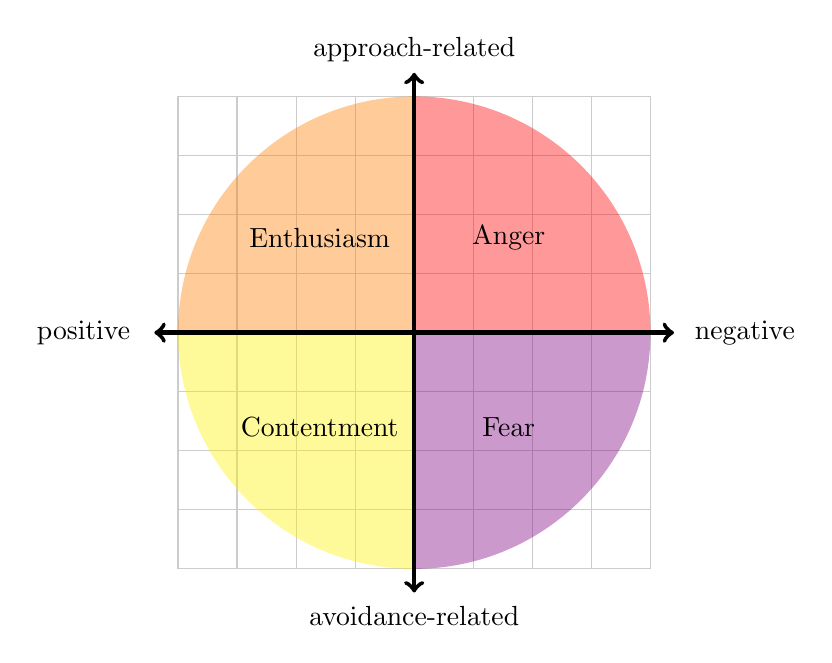
\begin{tikzpicture}[scale=3]
		\draw[step=0.25,black,thin,opacity=0.2] (-1,-1) grid (1,1);
		
		\fill [red, opacity=0.4] (1,0) arc [radius=1,start angle=0,end angle=90] -- (0,0);
											   
		\fill [violet, opacity=0.4] (0,-1) arc [radius=1,start angle=270,end angle=360] -- (0,0);
		
		\fill [orange, opacity=0.4] (0,1) arc [radius=1,start angle=90,end angle=180] -- (0,0);
		
		\fill [yellow, opacity=0.4] (-1,0) arc [radius=1,start angle=180,end angle=270] -- (0,0);
									   
		%\fill [violet, opacity=0.3] (0.95,-0.95) rectangle (0,0);
		%\fill [orange, opacity=0.5] (-0.95,0.95) rectangle (0,0);
		%\fill [yellow, opacity=0.5] (-0.95,-0.95) rectangle (0,0);
		
		\draw [ultra thick, <->] (-1.1,0) --(1.1,0);
		\draw [ultra thick, <->] (0,1.1) --(0,-1.1);
		\node at (0.4,0.4) {Anger};
		\node at (0.4,-0.4) {Fear};
		\node at (-0.4,0.4) {Enthusiasm};
		\node at (-0.4,-0.4) {Contentment};
		
		\node at (1.4,0) {negative};
		\node at (-1.4,0) {positive};
		\node at (0,1.2) {approach-related};
		\node at (0,-1.2) {avoidance-related};
	\end{tikzpicture}
	\caption{Emotions evoked by the \textsc{PSBC}.The left half contains the positive emotions of enthusiasm and contentment, whereas the right contains the negative emotions of anger and fear. Enthusiasm and anger are both approach-related, causing action, whereas contentment and fear are approach-related, causing flight or abstinence from action.}
	\label{fig:PSBC}
\end{figure}

In terms of implementation, this is realized via the system we saw in Figure~\ref{fig:affectiveSubsystem}, Section~\ref{sec:selectedSubsystems}: each of the four emotions has a \textsc{selector} reads percepts and the \textsc{hormone storage}, using them to decide whether and how intensely to activate and emotion. Emotions, once active, flow into the \textsc{hormone storage} and send messages into the global message space. The scheme is illustrated in Figure~\ref{fig:PSBC_system}: the filters of each emotions continually check the agent's percepts for relevant data. If a filter is activated, the message is passed the component's interpreter (to determine its urgency), which hands it to the processor. It then puts the message ``I feel emotion $E$ with intensity $\pi_E$'' into the message space. In this, it takes the \textsc{hormone storage} into account: experiencing an emotion increases the corresponding hormone level, and, conversely, a high hormone level intensifies the emotion. Formally, the hormone storage is defined thus:

\begin{definition}[Hormone storage]
	Let $E_1,\dots,E_n$ be the names of emotions. A hormone storage for the emotions $E_1,\dots,E_n$ is the ADT $\type{H}_n = \tuple{h_1 :: \R, \dots, h_n :: \R}$, together with the functions $\field{receive} :: \type{H}_n \rightarrow \N \rightarrow \R \rightarrow \type{H}_n$ and $\field{tick} :: \type{H}_n \rightarrow \type{H}_n$, given by
	
	$$
		\begin{array}{r c l}
			\field{receive}(h,e,\pi) & = & 2\pi * \log_2(1-\field{get}(h,e))\\
			\\
			\field{tick}(h) & = & \langle \field{get}_1(h) - 2\log(\field{get}_1(h)),\\
							 &   & \ \ \dots\\
							 &   & \ \field{get}_n(h) - 2\log(\field{get}_n(h)) \rangle.
		\end{array}
	$$
\end{definition}

The idea is that hormone level increases and decreases logarithmically: whenever an agent receives a message about an experienced emotion $e$ with intensity $\pi$, the corresponding level $h_e$ is increased proportionally to $\pi$ and the logarithm of the current level. The levels also decay at each time step, returning the agent to a neutral state over time if no stimuli are experienced.

One objection might be that, while an agent can experience conflicting emotions if multiple components are activated, different emotions cannot directly interact with each other. This is true; however, they can interact indirectly, through the message space: if a component $C_X$ reads the message of component $C_Y$ as a percept and, because of that, begins sending negatively-valenced messages, the emotion $X$ is effectively shutting down the emotion $Y$ --- even though the process is controlled by $C_Y$. I of course do not claim that this mechanism accurately reflects nature, that being an empirical question, but at the very least, it gives us a way to implement both ambivalence and quick mood changes.

\begin{figure}
	\centering
		\begin{tikzpicture}[scale=0.7,every node/.style={scale=0.7}]
		\figDataContainer{(0,0)}{Percepts}
		
		\draw [->] (2,0.3) -- (2,2) -- (-0.25,2) -- ++(0,1.05);
		\draw [->] (2,0.3) -- (2,2) -- (1.25,2) -- ++(0,1.05);
		\draw [->] (2,0.3) -- (2,2) -- (2.75,2) -- ++(0,1.05);
		\draw [->] (2,0.3) -- (2,2) -- (4.25,2) -- ++(0,1.05);
		                   
		\figFilter{(-0.75,4)}{$\ft{\mathsf{A}}$}
		\figFilter{(0.75,4)}{$\ft{\mathsf{F}}$}
		\figFilter{(2.25,4)}{$\ft{\mathsf{C}}$}
		\figFilter{(3.75,4)}{$\ft{\mathsf{E}}$}
		
		\draw [->] (-0.25,4) -- ++(0,0.5);
		\draw [->] (1.25,4) -- ++(0,0.5);
		\draw [->] (2.75,4) -- ++(0,0.5);
		\draw [->] (4.25,4) -- ++(0,0.5);
		
		\figProcessingComponentBentUp{(-0.75,6)}{$\int{\mathsf{A}}$}
		\figProcessingComponentBentUp{(0.75,6)}{$\int{\mathsf{F}}$}
		\figProcessingComponentBentUp{(2.25,6)}{$\int{\mathsf{C}}$}
		\figProcessingComponentBentUp{(3.75,6)}{$\int{\mathsf{E}}$}
		
		\draw [->] (-0.05,5.95) -- ++(0,0.55);
		\draw [->] (1.45,5.95) -- ++(0,0.55);
		\draw [->] (2.95,5.95) -- ++(0,0.55);
		\draw [->] (4.45,5.95) -- ++(0,0.55);
		
		\figProcessingComponent{(-0.75,7.5)}{$\fontsize{9.5pt}{1em}\proc{\mathsf{A}}$}
		\figProcessingComponent{(0.75,7.5)}{$\fontsize{9.5pt}{1em}\proc{\mathsf{F}}$}
		\figProcessingComponent{(2.25,7.5)}{$\fontsize{9.5pt}{1em}\proc{\mathsf{C}}$}
		\figProcessingComponent{(3.75,7.5)}{$\fontsize{9.5pt}{1em}\proc{\mathsf{E}}$}
		
		\draw [very thick, color=PaleRed,->] (-0.45,7.5) -- ++(0,0.5) -- ++(-1.75,0);
		\draw [very thick, color=PaleRed,-]  (1.05,7.5) -- ++(0,0.5) -- ++ (-1.5,0);
		\draw [very thick, color=PaleRed,-]  (2.55,7.5) -- ++(0,0.5) -- ++ (-1.5,0);
		\draw [very thick, color=PaleRed,-]  (4.05,7.5) -- ++(0,0.5) -- ++ (-1.5,0);
		
		\figDataContainer{(-6.5,8.8)}{Hormone storage}
		
		\draw [very thick, color=PaleRed,->] (-5.5,6.6) -- ++(0,-0.5) -- (-0.45,6.1) -- (-0.45,6.5);
		\draw [very thick, color=PaleRed,->] (-0.45,6.1) -- ++(1.5,0) -- ++(0,0.4);
		\draw [very thick, color=PaleRed,->] (1.05,6.1) -- ++(1.5,0) -- ++(0,0.4);
		\draw [very thick, color=PaleRed,->] (2.55,6.1) -- ++(1.5,0) -- ++(0,0.4);
		
		\draw [->] (-0.05,7.5) -- ++(0,1) -- (2,8.5) -- ++(0,1);
		\draw [->] (1.45,7.5) -- ++(0,1) -- (2,8.5) -- ++(0,1);
		\draw [->] (2.95,7.5) -- ++(0,1) -- (2,8.5) -- ++(0,1);
		\draw [->] (4.45,7.5) -- ++(0,1) -- (2,8.5) -- ++(0,1);
		
		\figDataContainer{(0,11.5)}{Message space}
		
	\end{tikzpicture}
	\caption{The PSBC as a collection of a hormone storage and four emotion selectors. The neural components shown are {\em anger} ($\mathsf{A}$), {\em contentment} ($\mathsf{C}$), {\em enthusiasm} ($\mathsf{E}$), and {\em fear} ($\mathsf{F}$).}
	\label{fig:PSBC_system}
\end{figure}

TODO: do the scrubber, which deletes anger-messages if "i am no longer angry"-messages get in.

\paragraph{Social judgement system.} The SJS has the task of recognizing other agents as such and guiding friendly and hostile interactions with them. Real social behaviour is very complex and involves not only other agents as individuals, but the group itself. In the minds of tribal animals, the group exists as an entity unto itself, with its own will and mood. Our agents will not implement this group dynamic. Instead, they will appraise each other agent individually, according to three criteria:

\begin{description}
	\item[Sympathy.] This determines how much an agent likes another one. Liked agents will receive friendly gestures, assistance in the form of food and protection from Wumpuses and hostile agents, disliked agents will be denied these benefits, receive hostile gestures and, if the dislike is sufficient, might be attacked.
	\item[Trust.] The trustworthiness of another agent influences the likelihood of two things: (1) the propensity to give out items in the hope of future reciprocation and (2) the aggressiveness if protection from the agent is present. The reasoning here is that the agent will be emboldened by the presence of trusted allies.
	\item[Competence.] Competence judges the capabilities of another agent. Competent agents will be respected, incompetent ones will be held in contempt. Similarly to trust, the presence of friendly, competent agents emboldens the agent.
\end{description}

Sympathy is the primary axis of judgement, since it determines whether others are seen as friends or enemies. Trust and competence are secondary and help an agents ascertain the quality of its allies an enemies. The three criteria are illustrated in Figure~\ref{fig:SJS}.

\begin{figure}

\end{figure}

\begin{figure}
	\centering
		\begin{tikzpicture}[scale=3]
		\draw [ultra thick, <->] (-1.1,0) -- (1.1,0);
		\draw [ultra thick, <->] (0,-1.1) -- (0,1.1);
		\draw [ultra thick, <->] ($({sqrt(2)/2}, {sqrt(2)/2})$) -- ($(-{sqrt(2)/2}, {-sqrt(2)/2})$);
		
		\node [left] at (-1.1,0) {trust};
		\node [right] at (1.1,0) {distrust};
		\node [below] at (0,-1.1) {contempt};
		\node [above] at (0,1.1) {respect};
		\node [below, right] at ($({sqrt(2)/2},{sqrt(2)/2})$) {sympathy};
		\node [above, left] at ($({-sqrt(2)/2},{-sqrt(2)/2})$) {antipathy};
	\end{tikzpicture}\\
	\caption{Emotions evoked by the SJS. The primary is axis is sympathy/antipathy, since it distinguishes friend from foe. Trust/distrust judges the loyalty/honor of another agent, whereas respect/contempt judges its competence.}
	\label{fig:SJS}
\end{figure}

\begin{figure}
	\centering
	\begin{tabular}{c}
	\textbf{\Large Enemy segment}\\
	\\
		\begin{tikzpicture}
	
		\cubeShape{(-1,-1)}{DeepRed} %tc
		\cubeShape{(0,-1)}{yellow} %uc
		\cubeShape{(-1,0)}{orange} %tr
		\cubeShape{(0,0)}{yellow} %ur
		
		\draw [ultra thick, <->] (-1.1,0) -- (1.1,0);
		\draw [ultra thick, <->] (0,-1.1) -- (0,1.1);
		\draw [ultra thick, <-] ($({sqrt(2)/2}, {sqrt(2)/2})$) -- (0,0);
		
		\coordinate (tc) at (-1,-1.3);
		\coordinate (uc) at (1.5,-1.2);
		\coordinate (tr) at (-1,1.2);
		\coordinate (ur) at (1.5,1.2);
		
		
		\node [left] at (tc) {\cubeLabel{Bumbling fool}{trust, contempt}};
		\node [right] at (uc) {\cubeLabel{Ineffectual villain}{distrust, contempt}};
		\node [left] at (tr) {\cubeLabel{Arch enemy}{trust, respect}};
		\node [right] at (ur) {\cubeLabel{Traitor}{distrust, respect}};
	\end{tikzpicture}
	
\\
	\end{tabular}
	
	\caption{The four antipathic judgements. Enemies can be respected or held in contempt, and deemed trustworthy or untrustworhty. Respect for an enemy implies that an agent holds it to be competent. Trust implies that an agent knows its enemy to be basically honourable.}
	\label{SJS_enemy}
\end{figure}

\begin{figure}
	\centering
	\begin{tabular}{c}
	\textbf{\Large Friend segment}\\
	\\
		\begin{tikzpicture}
	
		\cubeShape{(-1,-1)}{DeepGreen} %tc
		\cubeShape{(0,-1)}{green} %uc
		\cubeShape{(-1,0)}{RoyalBlue} %tr
		\cubeShape{(0,0)}{JungleGreen} %ur
		
		\draw [ultra thick, <->] ($({sqrt(2)/2},{sqrt(2)/2}) + (-1.1,0)$) --++ (2.2,0);
		\draw [ultra thick, <->] ($({sqrt(2)/2},{sqrt(2)/2}) + (0,-1.1)$) --++ (0,2.2);
		\draw [ultra thick, ->] ($({sqrt(2)/2},{sqrt(2)/2})$) --++ ($({-sqrt(2)/2}, {-sqrt(2)/2})$);
		
		\coordinate (tc) at (-1,-1.3);
		\coordinate (uc) at (1.5,-1.2);
		\coordinate (tr) at (-1,1.2);
		\coordinate (ur) at (1.5,1.2);
		
		
		\node [left] at (tc) {\cubeLabel{Lovable fool}{trust, contempt}};
		\node [right] at (uc) {\cubeLabel{Scamp}{distrust, contempt}};
		\node [left] at (tr) {\cubeLabel{Best friend}{trust, respect}};
		\node [right] at (ur) {\cubeLabel{Unreliable friend}{distrust, respect}};
	\end{tikzpicture}
	
\\
	\end{tabular}
	
	\caption{The four sympathic judgements. Friends, like enemies, respected or held in contempt, and deemed trustworthy or untrustworhty. Distrust renders the sympathetic judgement tentative, since the agent cannot be sure of the assistance of an untrustworthy friend. Contempt works similarly, but doubts a friend's ability, rather than loyalty.}
	\label{SJS_friend}
\end{figure}

With the help of the agent's memory, it delivers judgements about a given other agent.

\paragraph{Counterfactual perception.}

\paragraph{Attention-control.}

\paragraph{Decision-making.}

\paragraph{Memory.}

\paragraph{Relationship between components.}

\newpage



In this section, having sketched the underlying model and the relevant subsystems, I move on to the description of an implementation of an affective artificial agent. Its structure will necessarily be a gross simplification of any biological agent, but it will serve as a proof-of-concept.\\

\noindent
Note: instead of detailed partial descriptions, I, for now, sketch the rough outline of the proposed implementation to give a complete picture.

Outline of algorithm (provisional):

\begin{enumerate}
	\item One agent is composed of the following components:
		\begin{enumerate}
			\item Sensory perception
			\item Affect
			\item Planner and world simulator
			\item Memory
			\item Attention
		\end{enumerate}
	\item Sensory perception will be highly domain-dependent and, by necessity, simplified. Domains might be Blocks world or some custom-made game scenarios. In essence, it will deliver facts about objects and events in the world, bypassing the problem of faithfully implementing sight, hearing, smell, balance, pain, etc.
	\item At each step, sensory facts are put into the neural system's message space and are consumed by the evocative systems (PSBC, attention-refocusing, SJS, AS).
	\item The primitive parts of the PSBC can affect the executive system directly. Its higher-level parts, as well as the other three systems, work in the following way:
		\begin{enumerate}
			\item Attention-refocusing directs cognitive resources to stimuli it deems important. As a result, the priority of (certain) sensory messages is increased, increasing their influence on PSBC and the SJS.
			\item PSBC and the SJS evoke certain emotions. Thereby, they might set goals for the agent. This setting of goals engages the planner and world simulator, which try to devise a plan to meet said goal --- this is implemented via DLV-hex programs. These DLV-hex program, in turn, call the emotional systems in order to modulate both the planner and the world simulator according to the emotional state of the agent.
			\item Planned steps are committed to (short-term) memory.
		\end{enumerate}
	\item The PSBC's effects and the plans created by the agent are then translated into choices via conscious motor control, with the proviso that plans, even if deemed effective, are not executed under all circumstances: if some step is deemed too undesirable according to the emotional state of the agent at the time of execution, it might be abandoned and the planning stage starts anew. The kinds of actions that the agent executes are again highly dependent on the domain. Full physical simulation of a body would be prohibitively expensive, but simple, atomic actions like ``move left'' or ``attack'' would suffice for modelling purposes.
	\item The AS and sub-conscious motor control will not be implemented for the time being, as they are only relevant in highly sophisticated worlds.
\end{enumerate}